\documentclass[English,c,% 't' (resp. 'c') places text vertically at top/center of each slide
% PDF settings
hyperref={%
    pdftitle={FISA-DE2 OOP in Java},%
    pdfauthor={Muller, Gravier, Laforest, Subercaze},%
    pdfsubject={OOP in Java},%
    pdfkeywords={OOP, Java},%
    colorlinks=true,%
    urlcolor=blue,%
    linkcolor=%
    },%
% To load many pre-defined color names
xcolor={pdftex,svgnames} % dvipsnames, dvipsnames*, svgnames, svgnames*, x11names,
]{beamer}

\usetheme{Copenhagen}
%\setbeamertemplate{footline}[page number]
%\setbeamertemplate{frametitle}[default][center]
% To remove the navigation symbols from the bottom of slides:

% Remove navigation bar
\setbeamertemplate{navigation symbols}{}
% Remove outline at top
\setbeamertemplate{headline}{}

\addtobeamertemplate{navigation symbols}{}{%
    \usebeamerfont{footline}%
    \usebeamercolor[fg]{footline}%
    \hspace{1em}%
    \insertframenumber/\inserttotalframenumber
}

% Put text more on top of each slide for all slides
\addtobeamertemplate{frametitle}{}{\vspace*{-.7em}}

% Correct French/English indentation and splitting of words
\usepackage{babel}

% Correct management of accentuated chars in input file
\usepackage[utf8]{inputenc}

% Correct font for the generation of docs with accentuated chars
\usepackage[T1]{fontenc}      % Can handle hyphenation of words with accented characters
%%\usepackage[OT1]{fontenc}   % Might generated bad looking PDFs

% Insertion of images generated by external tools
\usepackage{graphicx}
% To generate pretty & scalable images directly in LaTeX
\usepackage{tikz}

% To print numbers correctly
\usepackage{numprint}

\usepackage[absolute,overlay]{textpos}

\usepackage{fourier}

\setbeamercovered{transparent}
\setbeamercovered{invisible}

\AtBeginSection[]
{
   \begin{frame}{Outline}
       \tableofcontents[currentsection]
   \end{frame}
}

\usepackage{url,manfnt}


% To be able to insert code listing
\usepackage{listings}

\definecolor{dkgreen}{rgb}{0,0.6,0}
\definecolor{gray}{rgb}{0.5,0.5,0.5}
\definecolor{mauve}{rgb}{0.58,0,0.82}

\lstset{frame=none,
  language=Java,
  aboveskip=1mm,
  belowskip=1mm,
  showstringspaces=false,
  columns=flexible,
  basicstyle={\tiny \ttfamily},
  numbers=left,
  numberstyle=\tiny\color{gray},
  keywordstyle=\color{blue},
  commentstyle=\color{dkgreen},
  stringstyle=\color{mauve},
  breaklines=true,
  breakatwhitespace=true,
  tabsize=2
}
\definecolor{algoTitle}{rgb}{0.84,0.83,0.94}

\usepackage{caption}
\DeclareCaptionFont{white}{\color{white}}
\DeclareCaptionFormat{listing}{\colorbox{algoTitle}{\parbox{\textwidth}{\bfseries #1#2 #3}}}
\captionsetup[lstlisting]{format=listing,labelfont=white,textfont=white}

\title[OOP in Java]{Object-Oriented Programming in \raisebox{-.3\height}{
\includegraphics[height=1.5em]{./images01/java_logo.png}}}
\logo{
\includegraphics[width=1cm]{images00/logo_tse.png}}
\author[Guillaume MULLER]{
  Guillaume \textsc{Muller}\\[1.2em]
  {\scriptsize \textit{based on work from:} \\[.1em]
    Ch. \textsc{Gravier}, F. \textsc{Laforest}, J. \textsc{Subercaze}}
}
\institute[TSE/UJM]{
  Télécom Saint-\'{E}tienne\\
  \medskip
  {\url{{pénom.nom}@univ-st-etienne.fr}}
}
\date[09/14/2020]{14~September~2020}

\begin{document}

%%%%%%%%%%%%%%%%%%%%%%%%%%%%%%%%%%%%%%%%%%%%%%%%%%%%%%%%%%%%%%%%%%%%%%
\begin{frame}
  \maketitle
\end{frame}

\section*{Maven}
%%%%%%%%%%%%%%%%%%%%%%%%%%%%%%%%%%%%%%%%%%%%%%%%%%%%%%%%%%%%%%%%%%%%%%
\begin{frame}[fragile]{\href{https://maven.apache.org/}{\color{white} Maven}\footnote{\url{https://dzone.com/refcardz/apache-maven-2}}}
  \begin{itemize}
    \item<1-> Goal: Manage compilation chain \& dependencies
    \bigskip
    \item<2-> Uses conventions\\
    \onslide<3-4>{
      \medskip
        \begin{itemize}
          \item<3-4> Project architecture
          \medskip
          \item<4> Pre-configured rules:\\
          \texttt{clean}, \texttt{compile}\ldots{}
        \end{itemize}
    }
    \bigskip
    \item<5-> Configuration via \texttt{pom.xml} file
    \bigskip
    \item<6-> Example usage:\\
    \texttt{mvn clean compile}
    \bigskip
    \item<7-> We will let Eclipse do (most of) that for us!!
  \end{itemize}

  \begin{textblock*}{0.4\linewidth}(6cm,3cm)%
    \onslide*<3-4>{
      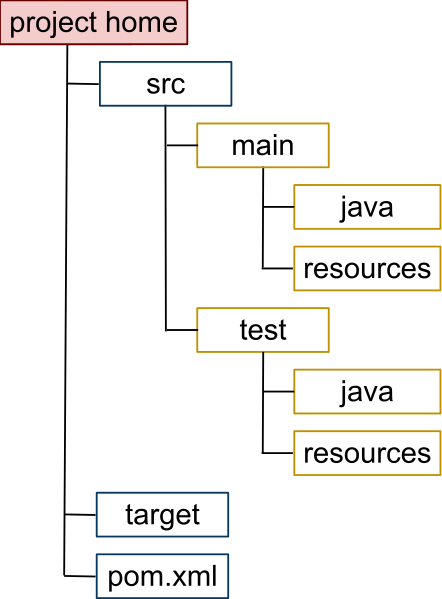
\includegraphics[width=3cm]{./images01/maven-project.png}
    }
  \end{textblock*}
  \begin{textblock*}{0.4\linewidth}(8cm,3cm)%
    \onslide*<4>{
      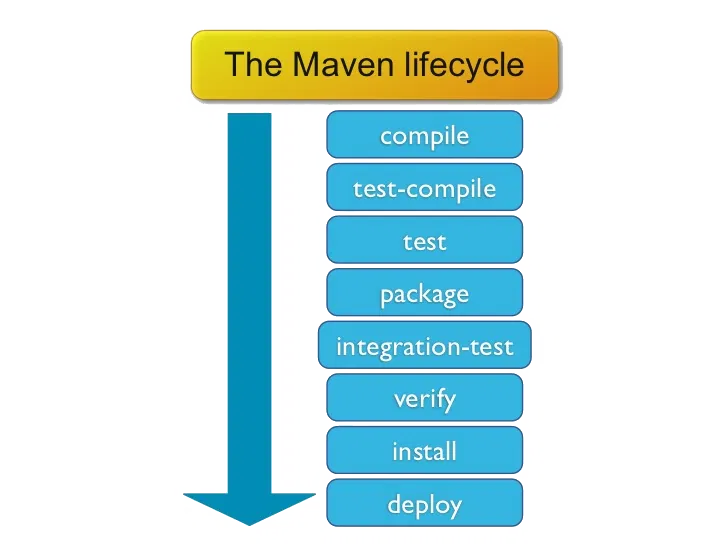
\includegraphics[width=6cm]{./images01/maven-lifecycle.png}
    }
  \end{textblock*}

\end{frame}

%%%%%%%%%%%%%%%%%%%%%%%%%%%%%%%%%%%%%%%%%%%%%%%%%%%%%%%%%%%%%%%%%%%%%%
\begin{frame}[fragile]{Maven -- Example \texttt{pom.xml} file}

  \begin{lstlisting}[language=xml,
    basicstyle={\tiny \ttfamily},
    keywordstyle={\color{dkgreen}},
    commentstyle={\color{dkgreen}},
    stringstyle=
    ]
    <project>
    <!-- model version is always 4.0.0 for Maven 2.x POMs -->
    <modelVersion>4.0.0</modelVersion>
    <!-- project coordinates, i.e. a group of values which uniquely identify this project -->
    <groupId>com.mycompany.app</groupId>
    <artifactId>my-app</artifactId>
    <version>1.0</version>
    <!-- library dependencies -->
    <dependencies>
    <dependency>
    <!-- coordinates of the required library -->
    <groupId>junit</groupId>
    <artifactId>junit</artifactId>
    <version>3.8.1</version>
    <!-- this dependency is only used for running and compiling tests -->
    <scope>test</scope>
    </dependency>
    </dependencies>
    </project>
  \end{lstlisting}

\end{frame}


\end{document}
